\documentclass{article}

\usepackage[utf8]{inputenc}
%\usepackage[english]{babel}
\usepackage[T2A]{fontenc}
\usepackage{tabularx}
\usepackage{amsmath,mathrsfs,amssymb}
\usepackage{bbding}
\usepackage{alltt}
\usepackage{epigraph}
\usepackage{verbatim}
\usepackage{soul}
\usepackage{latexsym}
\usepackage{array}
\usepackage{comment}
\usepackage{makeidx}
\usepackage{listings}
\usepackage{indentfirst}
\usepackage{verbatim}
\usepackage{color}
\usepackage{url}
\usepackage{xspace}
\usepackage{hyperref}
\usepackage{stmaryrd}
\usepackage{tikz}
\usetikzlibrary{arrows,decorations.pathreplacing,backgrounds,fit,positioning,shapes,chains,calligraphy,arrows.meta,shapes.arrows,overlay-beamer-styles}
\usepackage{euscript}
\usepackage{mathtools}
\usepackage{graphicx}
\usepackage{euscript}
\usepackage{mathtools}
\usepackage{transparent}
\usepackage{bold-extra}
\usepackage{subcaption}
\usepackage{placeins}
\usepackage{tikzsymbols}
\usepackage{amsthm}

\newcommand{\sembr}[1]{\llbracket{#1}\rrbracket}
\newcommand{\primi}[1]{\mathbf{#1}}
\newcommand{\Int}[2]{\primi{int}^{\mathcal {#1}}_{\mathcal {#2}}}
\newcommand{\Sem}[2]{\sembr{#1}_{\mathcal {#2}}}
\newcommand{\ph}{{\phantom{x}}}

\newcommand{\lama}{$\lambda\kern -.1667em\lower -.5ex\hbox{$a$}\kern -.1000em\lower .2ex\hbox{$\mathcal M$}\kern -.1000em\lower -.5ex\hbox{$a$}$\xspace}
\sloppy

\newcommand{\lang}[1]{\textsc{#1}}
\newcommand{\sys}[1]{\textsc{#1}}
\newcommand{\proc}[1]{\textbf{#1}}
\newcommand{\prog}[1]{\textbf{#1}}

\lstdefinelanguage{cc}{
basicstyle=\ttfamily\small,
keywords={include,int,char,float,double,long,short,void,static,volatile,auto,const,return,if,while,else},
keywordstyle=\rmfamily\bfseries,
sensitive=true,
}


\lstdefinelanguage{lama}{
keywords={ignore, ref, read, write, for, true, false, fun, case, of, esac, let, in, eta, skip, import, public, infix, infixl, infixr, at, before, after, syntax, var, val, if, then, else, elif, fi, do, while, od},
sensitive=true,
commentstyle=\small\itshape\ttfamily,
keywordstyle=\textbf,%\ttfamily\underline,
identifierstyle=\ttfamily,
basewidth={0.5em,0.5em},
columns=fixed,
mathescape=false,
fontadjust=true,
literate={->}{{$\to$}}3{=>}{{$\Rightarrow$}}3{=>>}{{$\Rightarrow$\hspace{-0.7em}$\Rightarrow$}}3,
morecomment=[s]{(*}{*)},
basicstyle=\normalsize
}

\lstdefinelanguage{plain}{
keywords={},
sensitive=true,
commentstyle=\small\itshape\ttfamily,
keywordstyle=\textbf,%\ttfamily\underline,
identifierstyle=\ttfamily,
basewidth={0.5em,0.5em},
columns=fixed,
mathescape=false,
fontadjust=true,
literate={->}{{$\to$}}3{=>}{{$\Rightarrow$}}3{=>>}{{$\Rightarrow$\hspace{-0.7em}$\Rightarrow$}}3,
morecomment=[s]{(*}{*)},
basicstyle=\normalsize
}

\lstset{
language=lama
}

\newtheorem*{lemma}{Lemma}

\begin{document}

\section{Semantics and Interpreters}

In this section we set the foundations for formal semantics which will be used in the rest of the course. We also discuss the
relation between programs and their representation in a concrete data domain, introduce the notion of interpreter and
consider some sample languages, their semantics and techniques for interpreter inplementations.

\subsection{Languages and Semantics}

We consider programming language $\mathcal L$ as a (countable) set of programs

\[
\mathcal{L}=\{p_1,\,p_2,\dots\}
\]

To give a \emph{semantics} for the language $\mathcal L$ is to specify two objects:

\begin{itemize}
\item a \emph{semantic domain} $\mathcal D$;
\item a \emph{total} mapping $\sembr{\bullet}^\ph_{\mathcal L} : \mathcal L \to \mathcal D$.
\end{itemize}

Thus, for a program

\[
p\in\mathcal L
\]

its semantics is just a

\[
\sembr{p}^\ph_{\mathcal L}\in\mathcal D
\]

When the language is easily deducible from the context we will omit the subscript and write simply $\sembr{\bullet}$.

By claiming the totality of $\sembr{\bullet}$ we 
make sure that any program has some semantics. The nature of semantic domain $\mathcal D$ essentially defines the nature of $\sembr{\bullet}_{\mathcal L}$;
for example, we can set

\[
\mathcal D=\{\Cat\}
\]

and (the only choice)

\[
\sembr{p}=\Cat
\]

for every $p\in\mathcal L$. We admit that this particular
semantics might not be very useful (this, however, depends on the nature of $\mathcal L$), but the important observations are that

\begin{itemize}
\item the choice of $\mathcal D$ has to be made;
\item there might be (and, \emph{as a rule}, are) multiple semantics for a given language.
\end{itemize}

These various semantics for a language may reflect its various properties (and we will see some of those in a little while); however, as a rule, one particular
semantics is chosen as the ``standard'' one.

\subsection{Data Domain}

If we speak of a general-purpose programming language and interested in its execution semantics then, probably, we may consider choosing the semantic domain
to be the set of all \emph{partially-recursive} functions and $\sembr{p}$ to be the function $p$ evaluates. This choice, however, would be too high-level and
abstract for our purposes.

To be more concrete, we first choose a \emph{data domain} $\mathfrak D$ to be the set of all reasonable data values the programs can take as inputs and
produce as outputs; then the semantic domain for executable semantics would be

\[
\mathcal{D}:\mathfrak{D}\to\mathfrak{D}
\]

Thus, executable semantics maps programs to data-processing functions.

In order to make further progress we stipulate the following properties of the data domain. First, we require its \emph{closedness under product}:

\[
\mathfrak{D}\times\mathfrak{D}\subset\mathfrak{D}
\]

In other words, $\mathfrak{D}$ contains all pairs, triples, etc. of its values.

The next requirement follows from out intention to make \emph{metaprogramming} possible. In short, the idea behind metaprogramming is
using \emph{programs} as \emph{data}. Indeed, all programming tools follow this approach: a compiler takes a program as input and
returns (another) program as output, etc. This can be done only if programs can be \emph{encoded} somehow in the data domain. We
consider some concrete encodings, using \lama data domain later; for now we assume that for arbitrary programming language $\mathcal{L}$
the set $\mathfrak{D}$ contains the \emph{representations}
of all programs in $\mathcal{L}$:

\[
\forall \mathcal{L}\; .\; \mathcal{L}\subset\mathfrak{D}
\]

We agreed above to consider programming languages as sets of programs; we could, equivalently, consider them as sets of \emph{representations} of
programs in some universal data domain. Since the correspondence between programs and their representations is one-to-one this convention would
not hinder any follow-up reasonings. From now on we will not distinguish programs (abstract objects) from their representations (concrete objects)
in $\mathfrak{D}$. Note, there can be miltiple representations within one data domain, but all of them are ``equivalent'' in the sense that
each pair of them admits an unambiguous conversions in both directions.

\subsection{Semantic Properties}

Let us have a language $\mathcal{L}$ and its \emph{two} semantics

\[
\begin{array}{rcl}
    \sembr{\bullet}^\ph & : & \mathcal{L} \to \mathcal{D}\\
  \sembr{\bullet}^\prime & : & \mathcal{L} \to \mathcal{D}
\end{array}
\]

with the \emph{same} semantic domain. We say that these semantics are \emph{equivalent} if and only if for arbitrary program $p\in\mathcal{L}$

\[
\sembr{p}^\ph=\sembr{p}^\prime
\]

In other words, equivalent semantics assign to each program in the language the same element of semantic domain. A question might arise why whould we
need two equivalent semantics; wouldn't the single one be sufficient? The answer is that, as we will see shortly, there are multiple ways of
describing semantics, and these different ways have different properties which make them preferrable in different settings. Sometimes it is desirable to
reformulate the semantics in different terms. By proving the equivalence between the two we can justify that we still deal with the language with the same
semantic properties.

Note, when the semantic domain is domain of functions $\mathfrak{D}\to\mathfrak{D}$, the equation above denotes the equality of functions: for
arbitrary $x, y\in\mathfrak{D}$

\[
\sembr{p}^\prime\,x=y \Leftrightarrow \sembr{p}\,x=y
\]

In other words, in both semantics $p$ is defined on exactly the same inputs and for each of these inputs it provides the same outputs.

Another important property is \emph{equivalence of programs} within the same semantics. We say that $p_1$ is (semantically) equivalent to $p_2$ if
and only if

\[
\sembr{p_1}=\sembr{p_2}
\]

Thus, equivalent programs have the same semantics. The equivalence of \emph{different} programs within the same semantics plays a crucial
role in justifying the correctness of program transformations. Let us have some transformation of programs into programs:

\[
f : \mathcal{L}\to\mathcal{L}
\]

We say that $f$ is \emph{semantically correct} if and only if for all programs $p$

\[
\sembr{f\,(p)}=\sembr{p}
\]

Thus, equivalent transformations do not change the semantics of programs; they can, however, change other their properties.

When the semantic domain is domain of functions, the equation above, again, denotes the equality of functions; additionally,
the following important notion can be introduced in this case. We say that $f$ is \emph{partially correct} if and only if
for all programs $p$ and all $x, y\in\mathfrak{D}$

\[
\sembr{p}\,x=y\Rightarrow\sembr{f\,(p)}\,x=y
\]

The difference between correctness and partial correctness is that in the former case the programs have exactly the same domain, while in
the latter the transformed program can be defined even if the original one in not. To some extent this is how
optimizing transformations work, as we've seen in the previos chapter.

Finally, there can be transformations between \emph{different} languages with the \emph{same} semantic domain. Let us have two languages $\mathcal{L}$ and $\mathcal{M}$
and let their semantics be

\[
\begin{array}{rcl}
  \sembr{\bullet}^\ph_\mathcal{L} & : & \mathcal{L}\to\mathcal{D}\\
  \sembr{\bullet}^\ph_\mathcal{M} & : & \mathcal{M}\to\mathcal{D}
\end{array}
\]

We say that a transformation

\[
f : \mathcal{L}\to\mathcal{M}
\]

is \emph{semantically correct} if and only if for all programs $p$

\[
\sembr{p}^\ph_\mathcal{M}=\sembr{f\,(p)}^\ph_\mathcal{L}
\]

And, again, when $\mathcal{D}$ is a domain of functions the equation above denotes the equality of functions, and the notion of
partial correctness arises. One example of transformation between languages is compiler; as we already know, compilers as a rule
are partially correct.


\subsection{Interpreters}

Let $\mathcal{L}$ and $\mathcal{M}$ be two languages, and

\[
\begin{array}{rcl}
\sembr{\bullet}^\ph_{\mathcal L} & : & \mathcal{L} \to \mathfrak{D} \to \mathfrak{D}\\
\sembr{\bullet}^\ph_{\mathcal M} & : & \mathcal{M} \to \mathfrak{D} \to \mathfrak{D}
\end{array}
\]

--- their semantics. An \emph{interpreter} for language $\mathcal{L}$, written in language $\mathcal{M}$, is a program $\Int{L}{M}\in\mathcal{M}$, such that for each
program $p^\ph_\mathcal{L}\in\mathcal{L}$ and each data value $x\in\mathfrak{D}$

\[
\sembr{\Int{L}{M}}^\ph_\mathcal{M}\,(p^\ph_\mathcal{L}\times x) = \sembr{p^\ph_\mathcal{L}}^\ph_\mathcal{L}\,(x)\eqno{*}
\]

To some extent an interpreter \emph{implements} a semantics for a programming language: given a program and its input, it provides exactly the same result
that this program calculates.

Now let's consider some tiny concrete language, its semantics and interpreter and see how these notions and approaches start working together.

\begin{figure}[t]
  \centering
  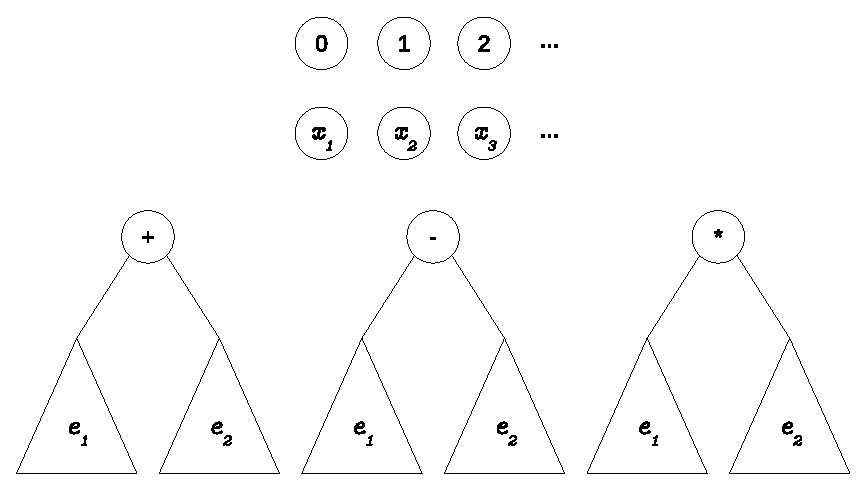
\includegraphics[scale=0.7]{images/02-01.eps}
  \caption{Abstract Syntax for Expression Language}
  \label{expression-syntax}
\end{figure}

\subsection{Simple Expression Language}

We start from describing so-called \emph{abstract syntax} of the expression language. We consider a countable set of \emph{variables}

\[
\mathscr{X}=\{x_1,\,x_2,\,\dots\}
\]

and a set of \emph{binary operators}

\[
\otimes=\{+,\,-,\,*,\,\dots\}
\]

which for now contains only symbols ``+'', ``-'', and ``*''. Then, the language of simple expressions $\mathcal{E}$ can be defined by
the following recursive scheme:

\[
\begin{array}{rcl}
  \mathscr{E} & = & \mathscr{X} \\
              &   & \mathbb{N} \\
              &   & \mathscr{E}\otimes\mathscr{E}
\end{array}
\]

This scheme defines a countable set of \emph{labeled ordered trees} of finite height: each node of such a tree is labeled, and for any node the order
of its immediate subtrees is essential. The simplest trees of this form are just leaves labeled with either variables or natural numbers; we simply
write $\mathcal{X}$ or $\mathbb{N}$ in the first two lines of definition of $\mathcal{S}$, but actually we mean tree nodes \emph{labeled} by the symbols of
these sets. As for the third line, it stipulates that for arbitrary two expressions $e_1,\,e_2\in\mathscr{E}$ a tree with a root labeled with any symbol
from $\otimes$ and immediate subtress $e_1$ and $e_2$ is also expression (see Fig.~\ref{expression-syntax}).

We call this definition \emph{abstract} syntax because it describes nothing more than a subordination between elementary constructs. In order to represent
expressions in some medium, however, we need \emph{concrete} syntax; it is easy to anticipate that there can be multiple concrete syntaxes for given
abstract one. In Fig.~\ref{expression-concrete} we give some examples of those for expressions: the first (\emph{a}) consists of graphical elements such as
circles, lines, texts, etc. Another one (\emph{b}) is the familiar \emph{infix notation} which includes numbers, letters, binary
operators and brackets. Yet another (but by no means the last one) is \emph{reverse Polish notation} (\emph{c}), in which binary operators are
put \emph{after} the operands they connect. In what follows we will stick with infix notation.

\begin{figure}[t]
  \centering
  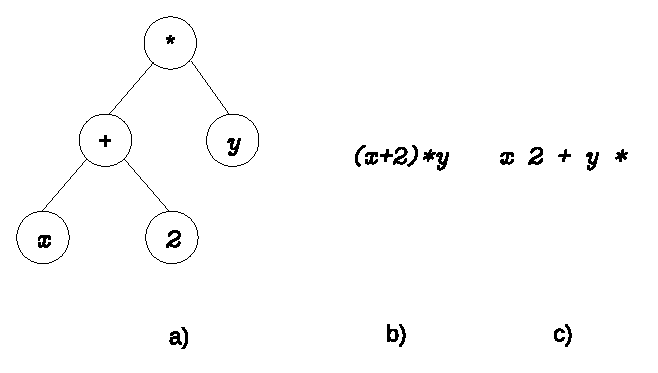
\includegraphics[scale=0.7]{images/02-02.eps}
  \caption{Various Concrete Syntaxes for Expression Language}
  \label{expression-concrete}
\end{figure}

Now we need to define the semantic domain for the semantics of simple expressions. We already hinted that this domain should be shaped like a set of some
data processing functions $\mathfrak{D}\to\mathfrak{D}$; however, we need to be more specific.

As we deal with arithmetic expressions it is rather natural to stipulate that the results of their evaluation are interger values, i.e. $\mathbb{Z}$ (as we agreed
earlier, we assume $\mathbb{Z}\subset\mathfrak{D}$); on the other hand, the value of an expression depends on the values of variables it contains. We can
encode these values as a \emph{state}~--- a function which maps variables to integer values:

\[
St : \mathscr{X} \to \mathbb{Z}
\]

There is nothing wrong with assuming $St\subset\mathfrak{D}$: as any expression can contain only finite number of variables we are interested only in
states with finite domains which can be encoded, for example, as finite lists of pairs. Thus, finally, we have the following ``type'' for the semantics
of simple expressions:

\[
\sembr{\bullet}^\ph_\mathscr{E}:\mathscr{E}\to(St\to\mathbb{Z})
\]

\subsection{Denotational Semantics of Simple Expressions}

There are multiple ways to give the semantics for a language formally. Here we use so-called \emph{denotational} way in which it is immediately
specified which object from the semantic domain corresponds to a given language construct. For this concrete language denotational semantics
looks simple and natural; however, for more advanced languages more advanced mathematical apparatus would be required. It is also worth mentioning that,
as a rule, denotational semantics gives us a very abstract, high-level view on the behavior of programs, which may or may not be desirable from
practical standpoint.

The denotational semantics for simple expression language is shown in Fig.~\ref{se-denot}.


\begin{figure}[t]
\[
\begin{array}{rcl}
  \sembr{z}^\ph_\mathscr{E} & = & \sigma \mapsto z \\  
  \sembr{x}^\ph_\mathscr{E} & = & \sigma \mapsto \sigma\,x \\
  \sembr{e_1\otimes e_2}^\ph_\mathscr{E} & = & \sigma \mapsto \sembr{e_2}^\ph_\mathscr{E}\,\sigma\oplus\sembr{e_2}^\ph_\mathscr{E}\,\sigma
\end{array}
\]
\caption{Denotational Semantics of Simple Expressions}
\label{se-denot}
\end{figure}

We give here three equations, one for each syntactic form of expression. In the right-hand side of each equation we immediately
give the object (a function from states to integers) which corresponds to the semantics of the expression in the
left-hand side. The notation $\star \mapsto \bullet$ is used to denote a function from $\star$ to $\bullet$; we refrain from
using the lambda notation since these functions belong to the meta-level, not to the object one.

In the first equation, when the expression is a natural number $z$, its semantics is a constaint function, which for
any state $\sigma$ return just this number $z$.

When the expression in question is a variable $x$, its semantics is a function which, given a state $\sigma$, returns
the value this state assigns to this variable.

Finally, when the expression is a binary operator with two subexpressions $e_1$ and $e_2$, its semantics is a function which, given a state $\sigma$,
first calcalates the values of subexpressions $e_1$ and $e_2$ in the same state, and then combines them using a certain arithmetic operator $\oplus$.
The correspondence between $\otimes$ and $\oplus$ is described by the following table:

\[
\begin{array}{ccl}
  \otimes & \oplus & \\
  \hline
  + & +      & \mbox{(integer addition)}\\
  - & -      & \mbox{(integer subtraction)}\\
  * & \cdot  & \mbox{(integer multiplication)}
\end{array}
\]

Note, while the symbols in the first and second columns look similar, they actually have different nature: the left ones are
elements of syntax while the right ones~--- conventional denotations for familiar arithmetic operators.
The last equation, thus, is actually a generic one which denotes three concrete equations in which $\otimes$ and $\oplus$ are
substituted coherently according to the table given above.

We can make two important observations.

First, in given semantics there is a single rule for any ``kind'' of expression (variable, constant, binary operation), and for each rule its right part defines
semantic function unambiguously. Thus, for each expression $e$ and each state $\sigma$ there is \emph{at most} one
integer number $y$ such that

\[
  \sembr{e}^\ph_\mathscr{E}\,\sigma=x
\]

This to some extent justifies our desire for $\sembr{e}^\ph_\mathscr{E}$ to be a function from states to integers. Indeed, the
property we just established is \emph{functionality}. On the other hand, in the domain of semantics the same property has
another name: \emph{determinism}. Thus, the semantics in question is deterministic, meaning that evaluating any expression in a given state
delivers at most one value. Non-deterministic semantics, according to which there can be multiple such values, seemingly are not
compatible with our framework of semantic functions; nevertheless, such semantics exist, and there are ways to fix this incompatibility.
Further we will deal only with deterministic semantics. 

Another important property is \emph{compositionality}: the semantics of a construct is expressed in the terms of the semantics
of its proper subconstructs. Indeed, the first two equations are \emph{axioms}, meaning, that no expressions containing semantic
brackets ``$\sembr{\bullet}^\ph_\mathscr{E}$'' occur in the right-hand side; the third equation is not an axiom, but semantic
backets are applied only to proper subconstructs ($e_1$ and $e_2$) of the construct in question ($e$). Compositionality is
a distinctive property of denotational semantics; using other semantic description styles may or may not result in compositional
semantic specification.

When a semantic is compositional, a certain proof principle~--- \emph{structural induction}~--- can be used to establish
its properties. This technique is essentially a specific kind of mathematical induction applied to \emph{finite trees} rather than to
natural numbers. To prove by structural induction that some property holds for all trees on needs to prove, first, that this
property holds for all leaves (\emph{base of induction}); then, assuming that the property holds for all trees up to a certain
height (\emph{induction hypothesis}) one needs to prove that the property holds for all trees one level higher. We demonstrate
the application of this principle by the following example.

We are going to prove the \emph{strictness} property of given semantics. It informally means that in order to calculate the
value for the whole expression one needs to calculate the values for all its subexpressions. First, we define the
following relation ``$\preceq$'' of one expression being a subexpression of another:

\[
\begin{array}{c}
  e^\prime \preceq e^\prime\otimes e \\
  e^\prime \preceq e\otimes e^\prime \\
  e\preceq e \\
  e^\prime\preceq e^{\prime\prime} \wedge e^{\prime\prime}\preceq e \Rightarrow e^\prime\preceq e
\end{array}  
\]

The first two lines define the \emph{immediate} subexpression relation while the last two~--- its \emph{reflexive-transitive}
closure. For example, for the expression $(x+2)*y$ all its subexpression are $(x+2)*y$, $x+2$, $y$, $x$, and $2$. 

\begin{lemma}[Strictness]
  For all $e$, $\sigma$ and $x$ if

  \[
  \sembr{e}^\ph_\mathscr{E}\,\sigma=x
  \]

  then for all $e^\prime\preceq e$ there exists $x^\prime$ such that

  \[
  \sembr{e^\prime}^\ph_\mathscr{E}\,\sigma=x^\prime
  \]
\end{lemma}
\begin{proof}
  For base case (variable and constant) the lemma holds vacuously since in both cases
  the only possible subexpressions are these expressions themselves.

  Assume the lemma holds for $e_1$ and $e_2$; we need to prove it holds for $e_1\otimes e_2$.
  By the definition of ``$\preceq$'' for any $e^\prime\preceq e_1\otimes e_2$ one of the
  following is true:

  \begin{enumerate}
  \item $e^\prime=e_1$, or
  \item $e^\prime=e_2$, or
  \item $e^\prime\preceq e_1$, or
  \item $e^\prime\preceq e_1$.
  \end{enumerate}

  By the condition of lemma we have $\sembr{e_1\otimes e_2}^\ph_\mathscr{E}\,\sigma=x$.
  By the definitiono of $\sembr{\bullet}^\ph_\mathscr{E}$ we have $\sembr{e_1}^\ph_\mathscr{E}\,\sigma\oplus\sembr{e_2}^\ph_\mathscr{E}\,\sigma=x$.
  By the definition of $\oplus$ there exist $x_1$ and $x_2$ such that

  \[
  \begin{array}{rcl}
    \sembr{e_1}^\ph_\mathscr{E}&=&x_1\\
    \sembr{e_2}^\ph_\mathscr{E}&=&x_2
  \end{array}
  \]

  If $e^\prime=e_1$ or $e^\prime=e_2$ then the lemma follows immediately.
  If $e^\prime\preceq e_1$ (or $e^\prime\preceq e_2$) the induction hypothesis can be applied as we just have proven that
  both $e_1$ and $e_2$ have some values being evaluated in the state $\sigma$.
\end{proof}

The strictness property, in particular, means that 

\end{document}

